\chapter{Summary and additional work}\label{Future}
\section{Summary of contributions}
In chapter~\ref{introduction} this thesis explores the basic constructs of how animals interact in different types of swarms such as shoals of fish, murmurations of starlings, and ant colonies. The chapter examines how these biological swarms have been studied and modelled to produced autonomous multi-agent robotic systems. The evolution of swarming techniques from the early modelling and mimicking of the biological swarms has shown that metrics are needed to provide an understanding of how agent interactions change over time and how the swarming algorithms affect the resultant swarm structures.

The remainder of the section focuses on the major contributions of the research:

\begin{itemize}
\item Model/Simulator
\item Inter-agent magnitude metric/Swarm Types
\item Perimeter coordination
\item Concave Reduction
\item Flood filling
\end{itemize}

\subsection{Model/Simulator}
Earlier research has identified the use of field effects as being an effective method of modelling an agent's behaviour within a swarm. This has led to vector mathematics being the most prominent mathematical modelling tool in swarm theory. Field effect modelling through vector mathematics is discussed in chapter~\ref{chapter:methods}. This chapter also introduces a graduated field effect implementation for cohesion~(\autoref{sec:Cohesion1}) and repulsion~(\autoref{sec:Repulsion1}) this approach helps to reduce collisions. The model also applies an aggregate weighted model that allows the field effect algorithms to be tailored to create regular structures~(\autoref{methods:weightedModel}).

All of the experimental work in this thesis has been carried out using a simulator written specifically for this project. Chapter~\ref{chapter:simulator} discusses the simulation process and the object model used for the representation of the swarming agents. The chapter discusses the mathematical models that have been applied to the modelling. The chapter also discusses how the simulator is applied to the experiments and how the results are achieved. The simulator has been designed with a specific set of requirements for this thesis and it allows the modelled swarms to be analysed by creating aggregated simulation data sets. The datasets consist of each agent's \textit{inter-agent vector magnitudes}, inter-agent distances, and inter-agent relationships in the form of cohesion and repulsion vectors. The simulator is configurable in terms of allowing the weighted model and field effects defined in chapter~\ref{chapter:metric} to be visualised and allows the environmental parameters to be altered to achieve the required effects discussed throughout. The simulator, being based on an object model, has allowed two applications to be developed: a graphical setup environment to create simulation configurations and a command line based simulation tool to execute the experiments. The graphical tool is capable of running small simulations in a real-time mode but for large swarms a command line version is used which incorporates simulated time to ensure the accuracy of the simulation results. The simulator uses a discrete time model to capture and implement the models~(\autoref{sim:time}). 

\subsection{Inter-agent magnitude metric}
The application of swarms as a platform to solve problems has necessitated the need to understand how agents in a swarm can be distributed and how their movements can be coordinated efficiently. Chapter~\ref{chapter:metric} identifies the \textit{inter-agent vector magnitude} as being a suitable metric to measure a swarm's internal movements~(\autoref{section:MagnitudeDynamics}). 

%% \begin{figure}[H]
%% \begin{center}
%% 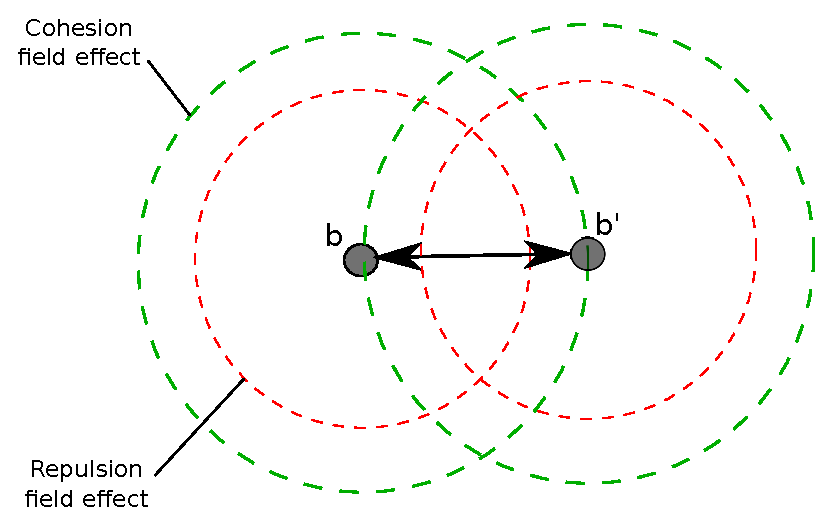
\includegraphics[width=9cm]{CHAPTER-9/figures/MagnitudeMetric1}
%% \end{center}
%% \caption{Magnitude Metric\label{additional:MagnitudeMetric1}}
%% \end{figure}

The chapter compares this new metric with the distance metric~(\autoref{section:DistanceDynamics}) currently in use and demonstrates how the \textit{inter-agent vector magnitude} is better suited to identifying the state of a swarm.  

%% \begin{figure}[H]
%% \begin{center}
%% \includegraphics[width=3cm]{CHAPTER-9/figures/DistanceMetric1}
%% \end{center}
%% \caption{Distance metric\label{additional:DistanceMetric1}}
%% \end{figure}

The \textit{inter-agent vector} metric is based upon the component vectors that determine the inter-agent interactions rather than the resultant distribution of the agents. This change of focus creates a transferable metric that allows the effect of any field effect based algorithm to be analysed independently of the resultant distributions that the field effects create. The new metric also allows the `hidden potential' of a swarm to be identified. Inter-agent distance distribution does not show the underlying `potential' with respect to an agent's current vector magnitude state. The new metric allows a swarm to be identified as being in a repulsive state such that it will expand over time or as being in a cohesive state which results in the swarm remaining a single entity with a tendency to `stick' together. The application and benefits of the new metric are discussed further in~\autoref{additional:MoreWork}.

In chapter~\ref{chapter:SwarmType} the effect of varying the field effects of a swarm's agents and the impact this has on the swarm's structure is examined. The chapter demonstrates how the field effects can be used to produce different types of swarms based upon inter-agent `visibility'. The chapter demonstrates how the swarm models can be analysed using both the distance metric and the new \textit{inter-agent vector metric} defined in chapter~\ref{chapter:metric}. The chapter demonstrates how identifying the underlying inter-agent interactions allows the type of swarm to be identified and also highlights improvements that can be made in the field effects model to improve a swarm's structure. 

\subsection{Perimeter coordination}
If the application of a swarm requires it to move in a specific direction then an additional attribute must be added to the field effect model to create a goal based characteristic. In chapter~\ref{chapter:coordination} alternative swarm co-ordination algorithms are presented to create goal-based swarms capable of being applied to reconnaissance type tasks. The alternate methods are compared to a baseline static swarm to identify the effects the algorithms have upon a swarm's structure. The comparisons are carried out using both the distance-based metric and the new \textit{inter-agent vector magnitude} metric. This thesis explores three basic approaches to implementing a goal based characteristic. All agents using their GPS modules, only perimeter based agents using their GPS modules, and finally using a subset of the perimeter selected using a simple counting technique. The findings in this chapter are that by reducing the number of coordinator agents in a swarm it is possible to maintain a stable internal structure whilst imposing a directional bias to a swarm. The most effective technique is to use the smallest subset of the perimeter by using the basic count algorithm~(\autoref{section:stabilityComparison1}). The algorithm that produced the most internal disturbance is the `all agents' algorithm where all agents are coordinators. The chapter also examines the effects of balancing the field effects on a pro-rata basis (number of coordinators) to reduce the negative effects the algorithms can introduce. This is achieved by adjusting the individual vector component weightings for each of the algorithms used~(\autoref{sec:AlternateBias1}). When the \textit{weighting movement direction} parameters are altered the basic count mechanism is still the most effective algorithm~(\autoref{fig:BaselineAllMag100-60-20-2}).

\subsection{Concave reduction}
Chapter~\ref{chapter:ConcaveReduction} examines how swarms can exhibit emergent behaviours from a simple algorithm. A localised algorithm is used to improve inter-agent distributions by identifying gaps between an agent's neighbours and moving the agent towards the gap. This simple change to the swarming model produces two behavioural changes. It causes a swarm to close voids and migrate towards a more uniform shape. These effects can be interpreted as a `healing' effect as they cause the swarm to be more uniform in shape with no internal anomalies. This can be useful when a swarm's structure is disrupted by a failed agent or from disruptions to a swarm's path. This behaviour can also be applied to encapsulating an object. The object encapsulation effect is presented in terms of an existing application area in the petrochemical industry where they have identified the use of swarms as a potential method of controlling oil spillages~(\autoref{voids:ObjectSurrounding}). The technique used in this thesis uses a Boid-based swarming approach which differs to the current research which uses an ant-colony-based approach. This `healing' behaviour is also applied to goal-based swarms in an attempt to remove voids in a reconnaissance based swarm when a swarm's path is disrupted~(\autoref{concave:mobileSwarm1}). The thesis demonstrates that the emergent behaviour is able to remove a void created by an obstacle improving the coverage of the swarm's path using the \textit{concave-reduction} effect.

\subsection{Flood filling}
In chapter~\ref{chapter:flooding} the cohesion and repulsion field effects (\textit{interaction vectors}) are used to create an area filling behaviour using a swarm of a fixed size. This is achieved by increasing the repulsion field effect of the agents to influence the distribution of the agents such that the agents fill a bounded area. The chapter examines two different techniques of coordinating the expansion process. The first technique involves using a `normal' swarm that uses both cohesion and repulsion to create a swarm that acts as a single entity and ensures agents maintain `visibility' of each of its neighbours. The second technique exploits the fact that the swarm is in a bounded area and removes the cohesion field effect and uses only the repulsion field to expand the agents throughout the space. The metrics discussed in chapter~\ref{chapter:metric} are used to identify the effects of the expansion on the swarm's internal structures and to identify terminating conditions for the filling behaviours.

\section{Future work}\label{additional:MoreWork}
The research in this thesis has investigated several issues with respect to swarm analysis but has also raised further questions that need to be answered. The new metric allows swarms to be analysed in a completely different way and has opened up the possibility of analysing new swarm configurations.

\subsection{Magnitude metric application}\label{additional:fieldsWork}
Swarms are often constructed from heterogeneous agents that adapt to stimuli but the agents themselves are usually modelled using homogeneous field effects. This modelling of homogeneous field effects lends itself to being measured and monitored by a distance based metric as discussed by Navarro et al. \cite{NIM:09} and Gazi et al. (\cite{SALGVPJ:08, VG:05, GP:02, GP:04, GP:04a, GP:05, GP:11}) due to the regular shapes and structures that emerge. The dependence on regularity of shapes and structures is a limitation of the distance metric due to the aggregation of the distances not reflecting the mathematical model that creates the structures. The magnitude based metric overcomes that limitation by analysing the vectors that effect the agent distribution. With heterogeneous field effects the inter-agent distances may vary in an equilibrium state due to the way the field effects overlap when agents interact. 

The \textit{inter-agent vector magnitude} metric takes into consideration the resultant effects of the mathematical model rather than just arbitrary distances between agents. The balancing of \textit{interaction vectors} affect the resultant agent distributions.

The additional work required here would be to identify potential applications of these variations in the field effects that could improve existing swarm applications. For example, if an agent is on a perimeter would the swarm benefit from reducing the field effects to create a greater compression effect? Would having a mixed field effect swarm produce better coverage of an area? What would be the impact of having variable field effects upon a goal-based swarm?

\subsection{Area flooding}
If agents could vary their field effects based on their position in a swarm (e.g. agents at the boundary) is it possible to improve coverage?

If agents were able to vary their field effects based on detected environmental features a swarm may be able to achieve set goals more efficiently in unknown environments. An environment may have narrow paths linking larger chambers. Allowing agents to change their field effects may allow a swarm to propagate through this type of environment more effectively. This application requires further work to identify the affectiveness of using adaptive field effects on area flooding.
 
\subsection{Path following and shape forming swarms}\label{sec:DirectionalShape1}
The \textit{destination vector} as discussed in~\autoref{sec:Direction1} has been based upon a swarm having a fixed single destination however this model can be changed slightly to produce two more possible swarming effects by applying the \textit{destination vector} to a set of points. The effects that are possible are to create swarms that form arbitrary shapes or a swarm that will migrate along a specific path. The \textit{destination vector} required to achieve these two emergent behaviours can be implemented using the coordination techniques discussed in chapter~\ref{chapter:coordination}.

The main area of research that is still required in this area is how to best implement the coordination. The thesis shows that changing how coordination is applied via perimeter coordinators can improve a swarm's structure however what is not know is what is the best way to apply the coordination if a swarm is being applied to a shape forming~\cite{EP:07} or path following task.

\subsection{Self optimisation}\label{sec:Optimisation1}
The research carried out in terms of improving the performance of a swarms internal distribution shows that as the parameters are changed it is possile to improve the performance of a swarm. Further work is therefore required to identify what optimisation techniques could be applied to a swarm's algorithms to create optimising swarm based on environmental conditions.

